%% --------------------------------------------------------------------
%% Template UTEC Tesis
%% --------------------------------------------------------------------
% Este es el archivo que se debe compilar.
% 
% Este template ha sido modificado y actualizado por Eduardo Castro y Roosevelt Ubaldo en base a lo trabajado por Víctor Murray, Oscar Ramos y Juan Carlos Barbaran.
%
% Última actualización: Mayo, 2022

\documentclass[a4paper,12pt,oneside]{tesisutec}

\selectlanguage{spanish}

%% Paquetes
\usepackage[utf8]{inputenc}
\usepackage[square, numbers, comma, sort&compress]{natbib}
% Libreria de idioma
\usepackage[spanish]{babel}
% Libreria para posicionamiento
\usepackage{float}
% Librerias para insertar codigos
\usepackage[spanish,onelanguage,ruled,vlined]{algorithm2e}
\usepackage{verbatim} 
% Librería para hipervínculos
\usepackage{hyperref}
 % Librería necesaria para arreglar el orden de referencias en overleaf.com
\usepackage{notoccite}

% Incluir acá los paquetes adicionales que deseas. 
% Ubicación de los imágenes.
\graphicspath{images/}

\makeatletter
% Reinsert missing \algbackskip
\def\algbackskip{\hskip-\ALG@thistlm}
\makeatother

\hypersetup{urlcolor=blue, colorlinks=true}

\begin{document}

\frontmatter

\department{...}
\degree{... }
\major{...}

\title{TÍTULO DEL TRABAJO DE INVESTIGACIÓN}

\author{Nombres y apellidos del alumno \orcid{0000-0000-0000-0000}} % Es obligatorio agregar ORCID del alumno
\supervisor{Nombres y apellidos de asesor \orcid{0000-0000-0000-0000}} % Es obligatorio agregar ORCID del asesor

\date{2022}

\maketitle

\setstretch{1.5}


\input{encabezados/dedicatoria}
\input{encabezados/agradecimientos}

\tableofcontents

\newpage

\listoftables

\newpage

\listoffigures

\addtocontents{toc}{\vspace{1.5em}}

%% ============================================================================
\mainmatter
\pagestyle{fancy}

\customchapter{RESUMEN}

El glioblastoma multiforme presenta una resistencia evolutiva que limita la duración del control logrado con temozolomida. Esta tesis propone GBMARL, un marco de aprendizaje por refuerzo multiagente adversarial que modela la terapia y la evolución tumoral como dos agentes que interactúan sobre un simulador de poblaciones sensibles y resistentes. La política de terapia se entrena con MAPPO bajo entrenamiento centralizado y ejecución descentralizada (CTDE), y se compara con IPPO, ausencia de tratamiento, dosis máxima tolerada y la heurística adaptativa de Gatenby.

El simulador se calibró integrando DepMap Public 26Q1 y GDSC2 release 8.5. El cruce recuperó 34 líneas de GBM con ensayos de sensibilidad y 24 con expresión completa. Para la temozolomida se obtuvo una brecha de sensibilidad aproximada de 9,1 veces entre las poblaciones sensible y resistente. La evaluación usa el tiempo a falla combinado, que termina cuando se supera el umbral de carga o cuando la fracción resistente alcanza la mayoría, registrando el modo de falla.

En la comparación nominal calibrada, quince políticas MAPPO alcanzaron una mediana de 34 días [27, 41] y superaron a Gatenby en 13/15 semillas; quince políticas IPPO alcanzaron una mediana de 31 días [23, 34] y superaron a Gatenby en 12/15. La diferencia pareada MAPPO--IPPO fue exploratoria ($p=0{,}013759$). El análisis de sensibilidad identificó una fragilidad importante frente a la reducción de $K$: con $K=0{,}8K_0$, la mediana de MAPPO cayó a 25 días. Por ello, los resultados constituyen evidencia \emph{in silico} de comportamiento adaptativo bajo el modelo especificado, no evidencia de eficacia clínica.

\noindent \textbf{Palabras clave:} glioblastoma; terapia adaptativa; resistencia evolutiva; aprendizaje por refuerzo multiagente; MAPPO-CTDE; temozolomida.

\customchapter{ABSTRACT}

\begin{center}
\large \vspace{-1.5cm} \textbf{Mitigating evolutionary resistance in glioblastoma using adversarial multi-agent reinforcement learning}
\end{center}

Glioblastoma multiforme develops evolutionary resistance that limits the duration of tumor control achieved with temozolomide. This thesis proposes GBMARL, an adversarial multi-agent reinforcement learning framework that models therapy and tumor evolution as two agents interacting over a simulator of sensitive and resistant tumor populations. The therapy policy is trained with MAPPO under centralized training and decentralized execution (CTDE), and is compared with IPPO, no treatment, maximum tolerated dose, and the adaptive Gatenby heuristic.

The simulator was calibrated by integrating DepMap Public 26Q1 and GDSC2 release 8.5. The data join recovered 34 GBM cell lines with sensitivity assays and 24 lines with complete expression data. For temozolomide, the estimated sensitivity gap between the sensitive and resistant populations was approximately 9.1-fold. Evaluation uses a combined time-to-progression endpoint: an episode ends when tumor burden crosses its control threshold or when the resistant fraction becomes a majority, while recording the failure mode.

In the nominal calibrated comparison, fifteen MAPPO policies achieved a median of 34 days [27, 41] and exceeded Gatenby in 13/15 seeds; fifteen IPPO policies achieved a median of 31 days [23, 34] and exceeded Gatenby in 12/15 seeds. The paired MAPPO--IPPO difference was exploratory ($p=0.013759$). Sensitivity analysis identified a major fragility to reductions in carrying capacity $K$: at $K=0.8K_0$, the MAPPO median fell to 25 days. The results therefore provide in-silico evidence of adaptive behavior under the specified model, not evidence of clinical efficacy.

\noindent \textbf{Keywords:} glioblastoma; adaptive therapy; evolutionary resistance; multi-agent reinforcement learning; MAPPO-CTDE; temozolomide.
 
\customchapter{INTRODUCCIÓN}

\introsection{Presentación del tema de investigación}

El glioblastoma multiforme (GBM) es uno de los tumores cerebrales primarios más agresivos en adultos. A pesar del tratamiento multimodal, la recaída es frecuente y la resistencia a los fármacos limita la duración del control logrado con temozolomida (TMZ)~\cite{Tan2020,Sipos2025,Adegboyega2021}. El protocolo de Stupp combina resección quirúrgica, radioterapia y TMZ, pero no elimina el problema evolutivo: las células con mayor tolerancia al tratamiento pueden expandirse durante la terapia~\cite{Stupp2005,Jezierzanski2024}.

La terapia adaptativa propone controlar el tumor sin ejercer una presión selectiva innecesariamente intensa. Su principio es conservar una población sensible que compita con las células resistentes, modulando la dosis según la evolución del sistema~\cite{Gatenby2022,Gallaher2017,Strobl2020}. Este enfoque no busca prometer una curación en un modelo reducido, sino estudiar si es posible retrasar el momento en que el tumor deja de ser controlable o tratable.

Esta tesis estudia ese problema mediante GBMARL, un marco de aprendizaje por refuerzo multiagente adversarial. En el modelo, un agente de terapia decide la dosis de TMZ y un agente tumoral modifica la transición fenotípica de células sensibles a resistentes. Ambos interactúan sobre un simulador dinámico de dos poblaciones tumorales, y la política de terapia se aprende mediante MAPPO con entrenamiento centralizado y ejecución descentralizada (CTDE).

\introsection{Descripción de la situación problemática}

Los modelos computacionales de dosificación suelen tratar la evolución tumoral como una dinámica fija o evaluar el éxito únicamente por la reducción inmediata de la carga. Esa simplificación puede favorecer a la dosis máxima tolerada (MTD): reduce el tumor al inicio, pero elimina la competencia sensible y puede acelerar la dominancia resistente. Por otro lado, las heurísticas adaptativas incorporan una intuición evolutiva útil, aunque no optimizan explícitamente sus decisiones ni representan al tumor como un adversario que aprende.

El problema de investigación consiste, por tanto, en diseñar y evaluar un entorno donde la terapia y la respuesta evolutiva del tumor estén acopladas, y donde la métrica de éxito refleje la duración del control clínicamente relevante. Para evitar que una estrategia sea premiada por mantener una carga baja cuando ya es predominantemente resistente, la tesis emplea el tiempo a falla combinado (TTP-combinado): el episodio termina por progresión de carga o por mayoría resistente, y registra cuál de los dos eventos ocurrió primero.

\introsection{Formulación del problema}

La pregunta central es:

\begin{quote}
\emph{¿En qué medida un marco de aprendizaje por refuerzo multiagente adversarial, entrenado sobre un simulador de GBM calibrado con datos reales de sensibilidad a TMZ, permite descubrir políticas de dosificación adaptativa que retrasen la intratabilidad frente a la MTD y a la heurística de Gatenby, y qué aporte adicional ofrece el crítico centralizado frente al aprendizaje independiente?}
\end{quote}

La comparación se formula como una evaluación \emph{in silico}. La calibración usa datos de sensibilidad farmacológica de GDSC2 y anotación de líneas celulares de DepMap; no pretende convertir esos datos \emph{in vitro} en evidencia clínica individual. Los parámetros que no están identificados por esas fuentes se mantienen como supuestos explícitos del modelo y se someten a análisis de sensibilidad.

\introsection{Objetivos de investigación}

\subsection*{Objetivo general}

Diseñar y evaluar GBMARL para descubrir políticas de dosificación adaptativa contra la resistencia evolutiva del GBM, utilizando un simulador de dinámica sensible--resistente calibrado con datos reales y una métrica de tiempo a falla combinado.

\subsection*{Objetivos específicos}

\begin{enumerate}
  \item Construir un simulador de dos poblaciones tumorales acoplado a la farmacodinámica de TMZ, y derivar la potencia relativa del fármaco a partir de datos de GDSC2 cruzados con DepMap~\cite{GDSC,DepMap}.
  \item Implementar un entorno multiagente con observabilidad parcial para la terapia, un agente tumoral adversarial y entrenamiento MAPPO-CTDE, junto con una variante IPPO para la ablación.
  \item Comparar las políticas aprendidas con ausencia de tratamiento, MTD y la heurística de Gatenby mediante TTP-combinado y modo de falla.
  \item Estudiar la variabilidad entre semillas, la sensibilidad a parámetros y el efecto del crítico centralizado, reportando los límites de validez del resultado.
\end{enumerate}

\introsection{Justificación}

El valor de este trabajo es metodológico. Un simulador explícito permite separar la potencia farmacológica respaldada por datos de los supuestos sobre crecimiento, competencia y eliminación del fármaco. El juego adversarial permite evaluar si la política conserva su desempeño cuando la respuesta tumoral no es pasiva. Finalmente, TTP-combinado hace visible un error que una métrica aislada de carga ocultaría: una estrategia puede producir una carga pequeña y, al mismo tiempo, haber perdido la capacidad de controlar la población resistente.

El marco también ofrece un procedimiento reproducible para estudiar políticas adaptativas antes de cualquier consideración clínica. Sus resultados no sustituyen ensayos celulares, modelos animales ni estudios clínicos; ayudan a identificar hipótesis de dosificación, condiciones de fallo y parámetros que requieren mejor medición.

\introsection{Alcance y limitaciones / restricciones}

El estudio se restringe a un modelo no espacial de dos poblaciones, un único fármaco (TMZ), una dinámica determinista con integración RK4 y un entorno de horizonte finito. El agente de terapia observa carga total y concentración del fármaco, pero no la fracción resistente directamente; el agente tumoral controla una tasa acotada de transición fenotípica. La calibración vigente integra DepMap Public 26Q1 y GDSC2 release 8.5, con 67 líneas GBM catalogadas, 34 con ensayos de sensibilidad y 24 con expresión completa.

Las cifras actuales se obtuvieron con quince semillas por variante y 120\,832 pasos efectivos por corrida. Esta muestra permite estimar la dispersión del entrenamiento, pero no es suficiente para una afirmación clínica ni para establecer universalidad estadística. La sensibilidad muestra además que la ventaja nominal puede desaparecer bajo cambios desfavorables de la capacidad de carga $K$ o de otros parámetros. La variable de salud del paciente no se interpreta como clínicamente calibrada: requiere datos de toxicidad y una definición clínica validada antes de incorporarse como conclusión del estudio.

\chapter{REVISIÓN CRÍTICA DE LA LITERATURA}

Lorem ipsum dolor sit amet, consectetur adipiscing elit. Nulla nec porta neque. Curabitur cursus aliquam metus, id porttitor libero semper vel. Mauris risus metus, ultricies ut massa vitae, dignissim rhoncus arcu. Nam vulputate id sapien nec lacinia. Mauris non tempor est. Nam eget nunc augue. Morbi tincidunt leo at sapien finibus facilisis. Nullam commodo erat non tempor dictum.

Duis convallis mauris eros. Interdum et malesuada fames ac ante ipsum primis in faucibus. Suspendisse et pellentesque tortor. Vivamus porttitor, lorem non interdum lacinia, ligula libero euismod diam, in commodo ipsum nibh a dui. Donec erat metus, suscipit quis suscipit at, condimentum et nunc. Phasellus ac felis euismod lectus mollis laoreet vel vehicula lorem. Quisque tincidunt turpis tempus odio tempus, vel interdum turpis auctor. Duis nec vulputate massa. Suspendisse egestas quis turpis non dictum. Proin et ultricies leo. Mauris posuere sagittis blandit. Pellentesque scelerisque rhoncus justo, nec interdum ante. Praesent finibus dictum lacus in pellentesque.

Integer at lacus nisi. Proin eu elit mi. Proin interdum nulla vitae turpis tincidunt fermentum. Duis dui lorem, ornare vel metus sit amet, consequat lacinia ex. Cras ornare porta malesuada. Proin vehicula, velit a interdum malesuada, nulla diam accumsan urna, et efficitur ipsum mi id sapien. Vivamus accumsan aliquet leo ac interdum. Ut molestie purus a blandit ultricies. Aenean ornare eu mauris quis gravida. Nam molestie ullamcorper egestas. In hac habitasse platea dictumst. Nulla pulvinar orci tempor varius porttitor.

\section{Sección 1}

Lorem ipsum dolor sit amet, consectetur adipiscing elit. Cras scelerisque quis augue malesuada porttitor. Phasellus tincidunt ipsum quis metus pellentesque commodo. Phasellus vitae metus arcu. Pellentesque scelerisque ac nulla laoreet mollis. Vivamus blandit, velit eget convallis eleifend, nibh risus congue sapien, tristique bibendum justo lorem eget arcu. Quisque mollis tristique tellus, sit amet hendrerit purus lacinia id. Fusce sed nunc arcu. Phasellus porttitor convallis ipsum, sit amet tempus nulla mattis a \cite{Reumann2012}.

Sed eu orci feugiat, mollis nunc convallis, lobortis lorem. Suspendisse in lacinia magna, vel elementum tortor. Suspendisse hendrerit commodo justo, vitae posuere nisl eleifend at. Morbi vehicula risus ut diam tempus, ac dapibus erat euismod. Nunc quis elementum mi, et dictum nulla. Mauris rhoncus diam ac orci laoreet lobortis. Fusce et augue efficitur, dignissim dui ac, convallis est.



\section{Segundo subtítulo}

\subsection{División del segundo subtítulo}

En la actualidad, las unidades de información hacen frente a muchos cambios
debido a los avances tecnológicos, explosión informativa, nuevos recursos y
soportes, por lo cual se implementan servicios innovadores que les permitan a
sus usuarios tener acceso a muchas fuentes de información. Para asegurar el
acceso y uso de los servicios los usuarios requieren poseer una serie de
habilidades que les permitan identificar, recuperar, manejar, discernir,
organizar, utilizar y comunicar la información de manera eficaz para la toma de
decisiones. La relación entre $a$ y $b$ puede expresarse como
%
\begin{equation}
  \label{eq:1}
  a+b=\sqrt{\frac{4}{3}},
\end{equation}
%
donde $a$ y $b$ son escalares.

Entre las causas se pueden considerar la falta de tiempo asignado al taller,
las limitaciones en cuanto a laboratorios, el poco personal, la falta de una
correcta selección de los contenidos, así como, una calificación que asegure el
cumplimiento de los objetivos. Un ejemplo de cómo poner una figura se muestra en la Fig. \ref{fig:diagram2}, y es importante recordar la relación mostrada en \eqref{eq:1}.


\begin{figure} 
\begin{center}
\begin{tabular}{cc}

\includegraphics[height=3cm]{images/logo_utec.png} &

\includegraphics[height=2cm]{images/logo_utec.png} \\
(a) & (b)
\end{tabular}
\caption{\label{fig:diagram2}Scheme showing the architecture of a generic kinematic task. (a) Logo en tamaño de 3 centímetros. (b) Logo en tamaño de 2 centímetros.}
\end{center}
\end{figure}


\section{Tercer subtítulo}

\subsection{División del tercer subtítulo}

En la actualidad, las unidades de información hacen frente a muchos cambios
debido a los avances tecnológicos, explosión informativa, nuevos recursos y
soportes, por lo cual se implementan servicios innovadores que les permitan a
sus usuarios tener acceso a muchas fuentes de información. Para asegurar el
acceso y uso de los servicios los usuarios requieren poseer una serie de
habilidades que les permitan identificar, recuperar, manejar, discernir,
organizar, utilizar y comunicar la información de manera eficaz para la toma de
decisiones.

Entre las causas se pueden considerar la falta de tiempo asignado al taller,
las limitaciones en cuanto a laboratorios, el poco personal, la falta de una
correcta selección de los contenidos, así como, una calificación que asegure el
cumplimiento de los objetivos.

\begin{table}[H]
    \centering
    \begin{tabular}{c|c}
        Tiempo($s$) & Distancia($m$) \\
        \hline
        10 & 23 \\
        20 & 33 \\
        30 & 43 \\
        40 & 53 \\
    \end{tabular}
    \caption{Tiempos versus distancia.}
    \label{tab:tiempo_versus_distancia}
\end{table}
\input{secciones/capitulo2}
\input{secciones/capitulo3}
\chapter{RESULTADOS}
\label{cap:resultados}

Este capítulo presenta los resultados experimentales de GBMARL siguiendo el orden de construcción del marco: la calibración del simulador (Sección~\ref{sec:res-calibracion}), la validación del entorno y la convergencia del aprendizaje (Sección~\ref{sec:res-aprendizaje}), la comparación frente a las líneas base con la métrica auditada (Sección~\ref{sec:res-comparacion}), el mecanismo de la política aprendida (Sección~\ref{sec:res-mecanismo}), la ablación del crítico centralizado (Sección~\ref{sec:res-ablacion}), el análisis de sensibilidad (Sección~\ref{sec:res-sensibilidad}) y la robustez adversarial mediante explotabilidad (Sección~\ref{sec:res-explotabilidad}). La interpretación de estos hallazgos y sus implicaciones se desarrollan en el capítulo siguiente.

\textbf{Nota de estado.} Las cifras de esta revisión se distinguen entre resultados históricos y la auditoría calibrada del 8 de septiembre de 2026. La auditoría usa DepMap Public 26Q1, GDSC2 release 8.5 y la huella de parámetros \texttt{1fd8464abb97}; las tablas históricas que aún no fueron reejecutadas con esa huella se mantienen únicamente como referencia y no deben combinarse con los resultados nuevos.

\section{Calibración del simulador}
\label{sec:res-calibracion}

La corrección del cruce entre GDSC2 y DepMap mediante \texttt{SANGER\_MODEL\_ID} recuperó \textbf{34 líneas celulares de glioblastoma} con ensayos de sensibilidad a temozolomida, de las cuales \textbf{24} cuentan con anotación genómica completa. El catálogo DepMap contiene 67 líneas GBM; el valor 6 de la versión anterior era un artefacto del mapeo por nombre y no una limitación real del catálogo.

De los 24 modelos con expresión completa se derivó una concentración inhibitoria relativa de la población sensible $\mathrm{IC50}_S \approx 0{,}36$ y de la población resistente $\mathrm{IC50}_R \approx 3{,}27$, es decir, una brecha de sensibilidad de aproximadamente $9\times$. El techo de muerte celular se ancló al crecimiento mediante una constante de diseño documentada en el código, resultando en $\delta_S^{\max} = 0{,}30$ y $\delta_R^{\max} = 0{,}15$; estos dos valores no son mediciones clínicas directas. La calibración caracteriza la respuesta relativa del ensayo \emph{in vitro}, pero por sí sola no permite concluir sobre eficacia clínica. La Figura~\ref{fig:dynamics} muestra la dinámica de referencia del simulador calibrado bajo distintos regímenes de dosis.

\begin{figure}[H]
\centering
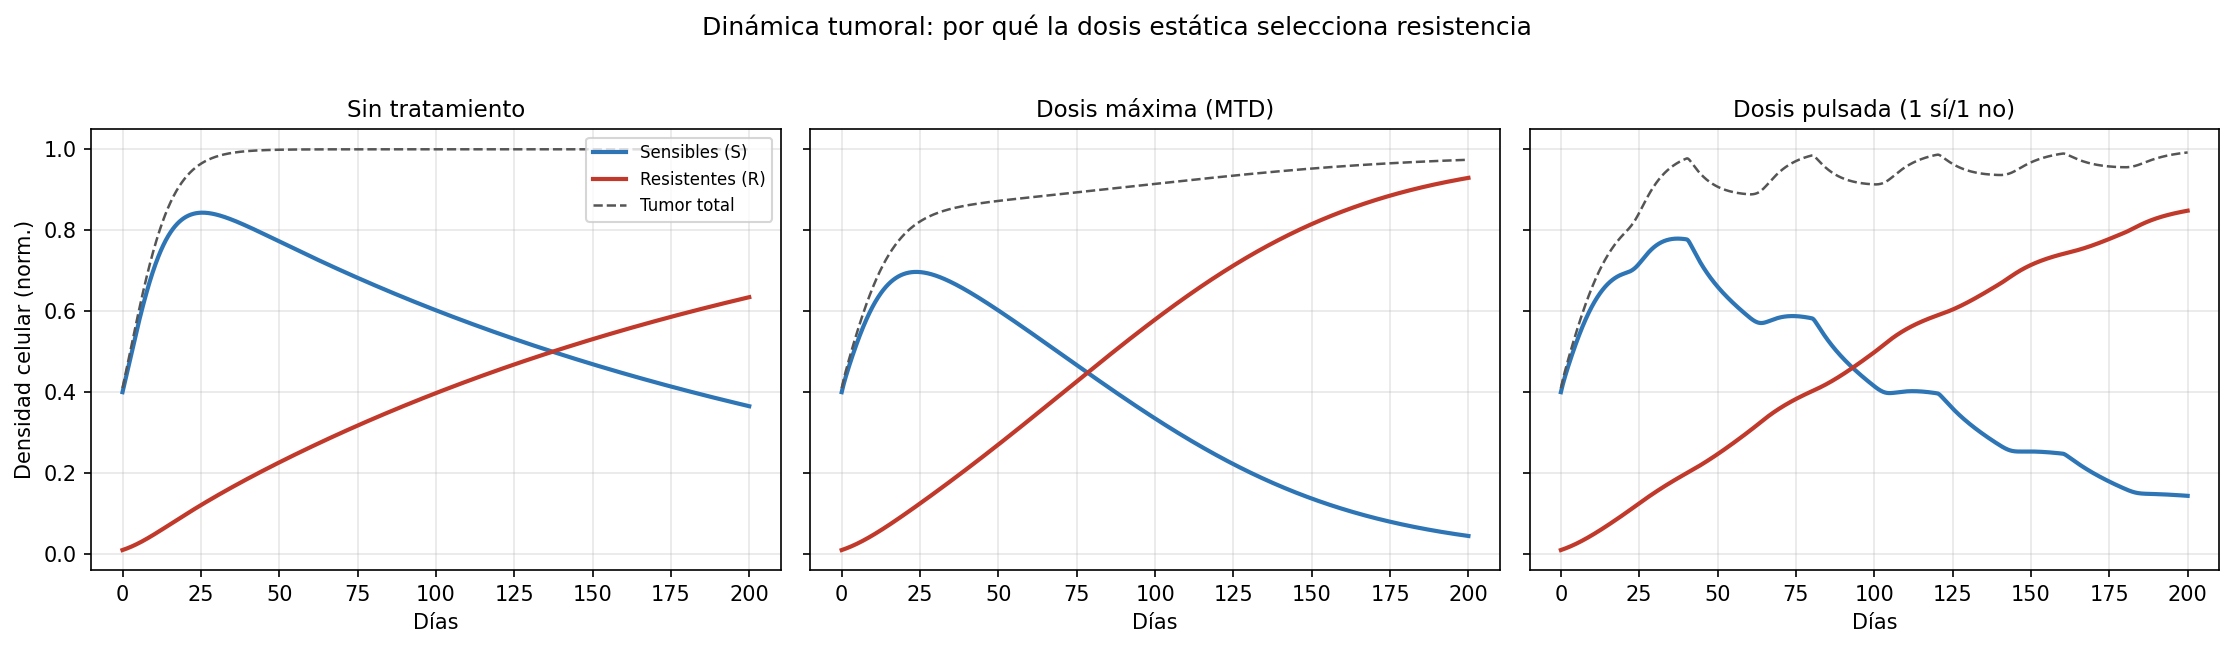
\includegraphics[width=0.85\textwidth]{images/dynamics_baseline.png}
\caption{Dinámica de referencia del simulador calibrado: evolución de las poblaciones sensible y resistente bajo distintos regímenes de dosificación.}
\label{fig:dynamics}
\end{figure}

\section{Validación del entorno y convergencia del aprendizaje}
\label{sec:res-aprendizaje}

Siguiendo la estrategia de validación incremental, se entrenó primero un agente único con PPO contra un tumor de comportamiento fijo. El retorno del agente de terapia mejoró de forma sostenida durante el entrenamiento, confirmando que el entorno es aprendible antes de introducir la complejidad multiagente.

Posteriormente, el entrenamiento adversarial por \emph{self-play} con MAPPO mostró la co-evolución de ambos agentes, como ilustra la Figura~\ref{fig:learning}. El régimen determinista garantiza que una misma semilla sea reproducible; no implica que todas las semillas converjan al mismo equilibrio. De hecho, la variabilidad entre inicializaciones es una limitación que se reporta explícitamente.

\begin{figure}[H]
\centering
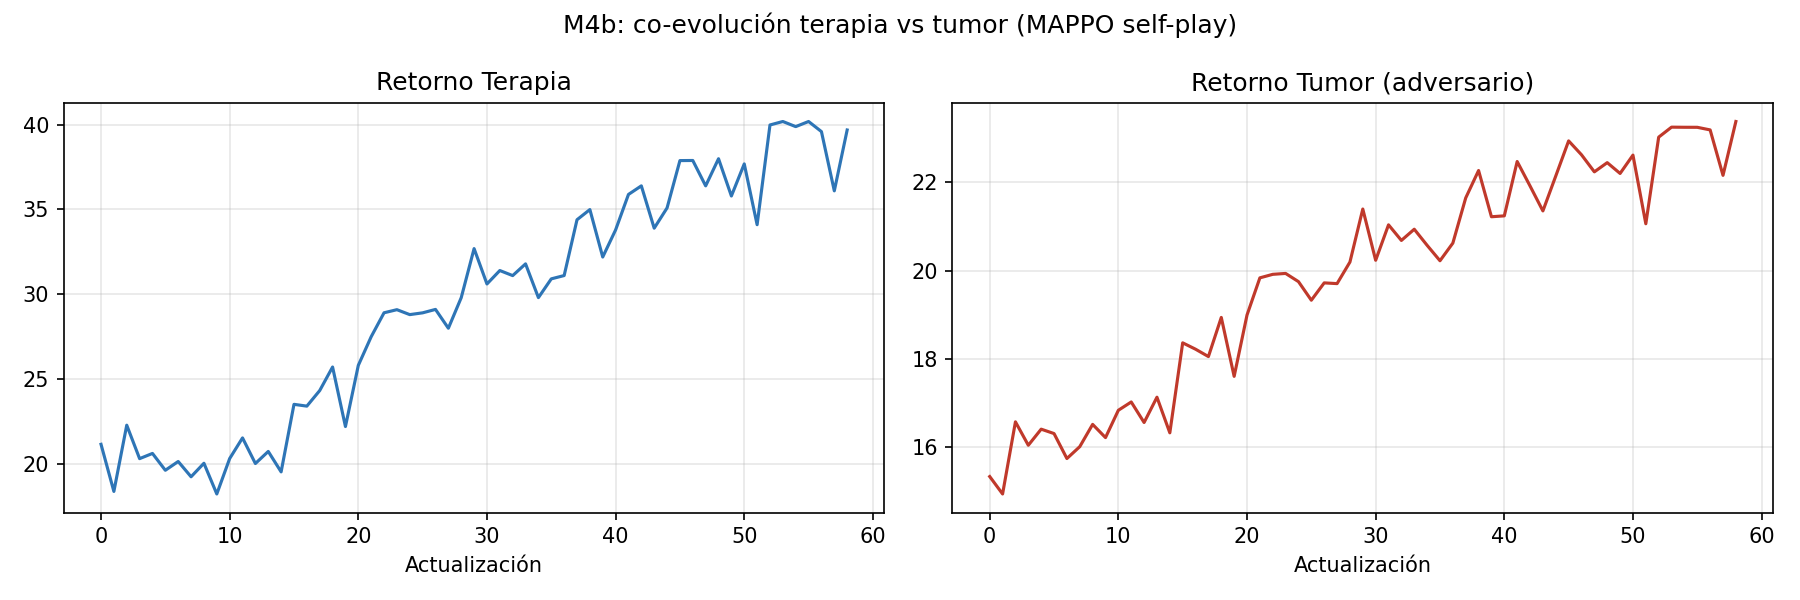
\includegraphics[width=0.95\textwidth]{images/mappo_learning_curves.png}
\caption{Curvas de aprendizaje del entrenamiento adversarial MAPPO por self-play: retorno del agente de terapia (izquierda) y del agente tumoral (derecha) a lo largo de las actualizaciones.}
\label{fig:learning}
\end{figure}

\section{Comparación frente a las líneas base}
\label{sec:res-comparacion}

La política aprendida se comparó contra tres referencias deterministas bajo la métrica de tiempo a falla combinado (TTP-combinado), reportando el modo de falla de cada estrategia. La Tabla~\ref{tab:res-baselines} resume los resultados de una evaluación representativa.

\begin{table}[H]
\centering
\caption{Comparación de estrategias bajo la métrica TTP-combinado, con el modo de falla. Métrica auditada mediante el procedimiento de diagnóstico.}
\label{tab:res-baselines}
\renewcommand{\arraystretch}{1.25}
\begin{tabular}{l|c|c|c|l}
\textbf{Estrategia} & \textbf{TTP (días)} & \textbf{Carga final} & \textbf{Frac.\ R final} & \textbf{Modo de falla} \\
\hline
Sin tratamiento     & 12  & 0.80 & 0.12 & carga progresó \\
MTD (dosis máx.)    & 13  & 0.09 & 0.52 & resistencia mayoría \\
Gatenby (adaptativa)& 27  & 0.38 & 0.53 & resistencia mayoría \\
MAPPO (aprendida)   & 41  & 0.79 & 0.51 & resistencia mayoría \\
\end{tabular}
\end{table}

Dos observaciones se desprenden de la Tabla~\ref{tab:res-baselines}. Primero, la métrica auditada revela que la ausencia de tratamiento falla por progresión de carga (día 12) mientras la fracción resistente permanece baja (0.12); todas las estrategias que tratan fallan, en cambio, por mayoría resistente. Segundo, la dosis máxima reduce la carga al mínimo (0.09) pero falla casi tan rápido como la ausencia de tratamiento (día 13), confirmando que la reducción agresiva del tumor precipita la resistencia. La política aprendida por MAPPO alcanza el mayor tiempo de manejo (41 días en esta corrida), superando a la heurística de Gatenby (27 días) y a la dosis máxima (13 días). La Figura~\ref{fig:ttp} muestra las trayectorias de carga tumoral y de fracción resistente para las cuatro estrategias.

\begin{figure}[H]
\centering
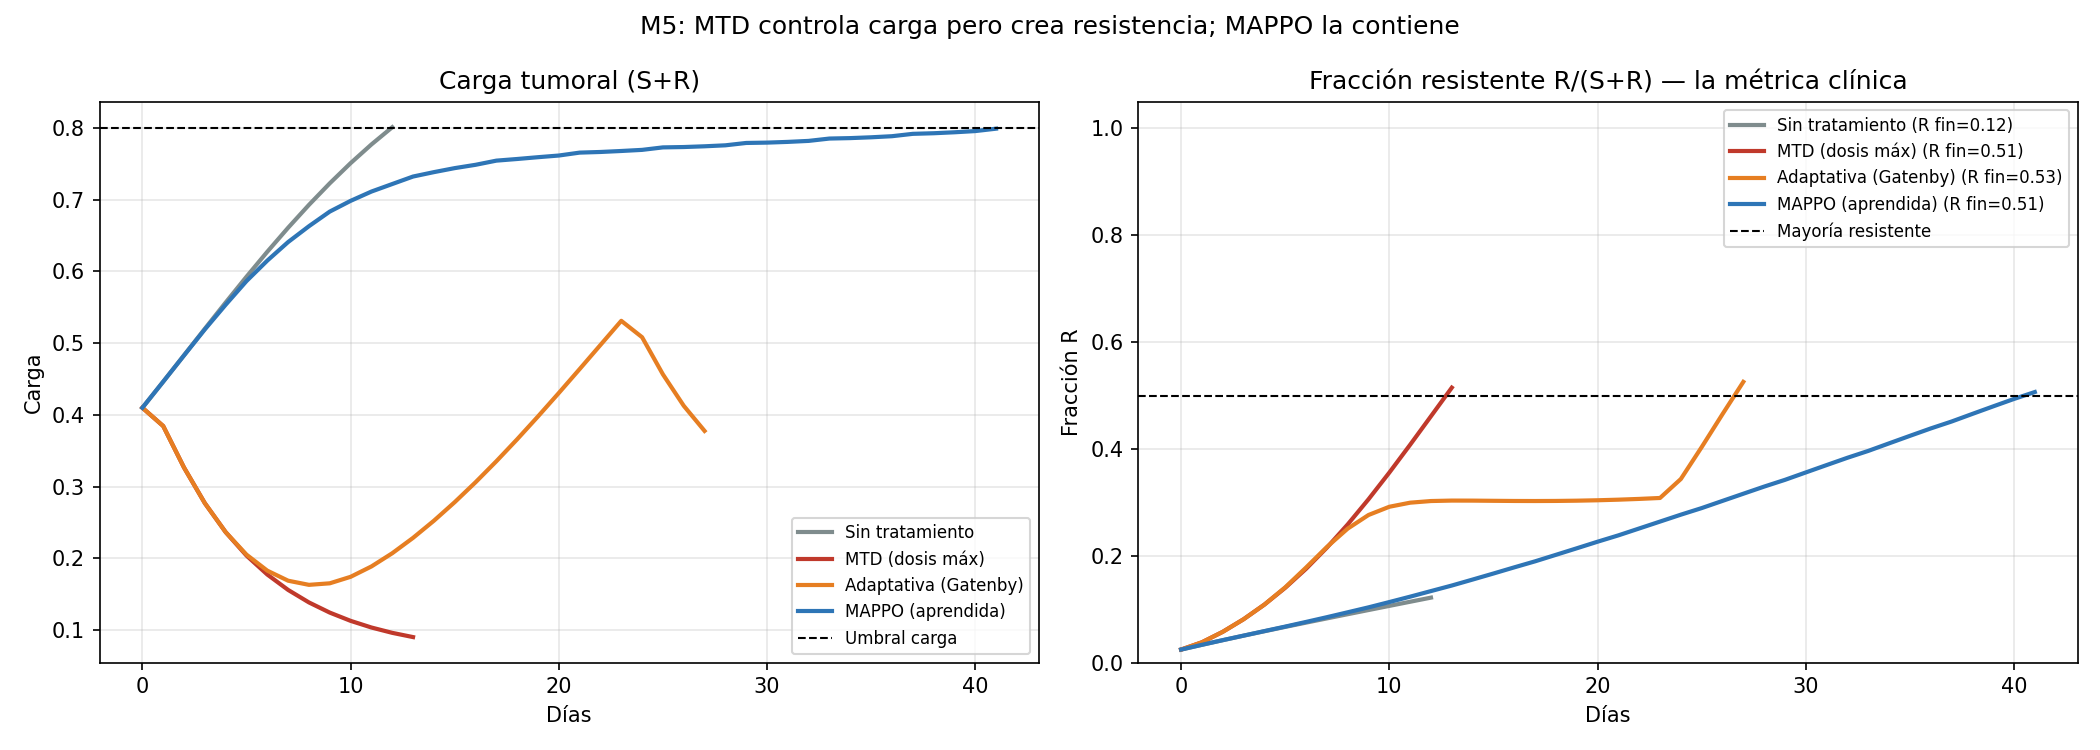
\includegraphics[width=0.95\textwidth]{images/evaluation_ttp.png}
\caption{Trayectorias de carga tumoral (izquierda) y de fracción resistente (derecha) para las cuatro estrategias. La dosis máxima controla la carga pero lleva la resistencia a su totalidad; la política aprendida retrasa la dominancia resistente.}
\label{fig:ttp}
\end{figure}

\subsection{Validación histórica multi-semilla y bimodalidad}

La corrida histórica del protocolo se evaluó sobre 15 semillas independientes. La distribución de los tiempos de manejo fue reportada como \textbf{bimodal}: una fracción de las corridas convergió a una cuenca con tiempos en el rango de 25 a 33 días, mientras que otra alcanzó una cuenca superior, en torno a los 41 días. Estas cifras pertenecen a una configuración anterior y no fueron revalidadas en la auditoría calibrada del 8 de septiembre de 2026; se conservan aquí como referencia metodológica, no como evidencia nueva.

Las afirmaciones de significancia de esta corrida histórica no deben transferirse automáticamente a la auditoría actual. La comparación calibrada nueva, con quince pares, se reporta en la Sección~\ref{sec:res-confirmacion}. La Figura~\ref{fig:validation} corresponde a la corrida histórica.

\begin{table}[H]
\centering
\caption{Validación histórica multi-semilla ($n=15$) del TTP-combinado. Las líneas base son deterministas. Esta tabla no corresponde a la auditoría calibrada del 8 de septiembre de 2026.}
\label{tab:res-multisemilla}
\renewcommand{\arraystretch}{1.25}
\begin{tabular}{l|c|c}
\textbf{Estrategia} & \textbf{TTP (días)} & \textbf{Significancia} \\
\hline
MTD (dosis máx.)     & 13                       & --- \\
Gatenby (adaptativa) & 27                       & --- \\
MAPPO (mejor corrida)& 41                       & --- \\
MAPPO (media, $n=15$)& $33{,}5 \pm 5{,}8$ (mediana 32) & $p<0{,}001$ vs.\ MTD y Gatenby \\
\end{tabular}
\end{table}

\begin{figure}[H]
\centering
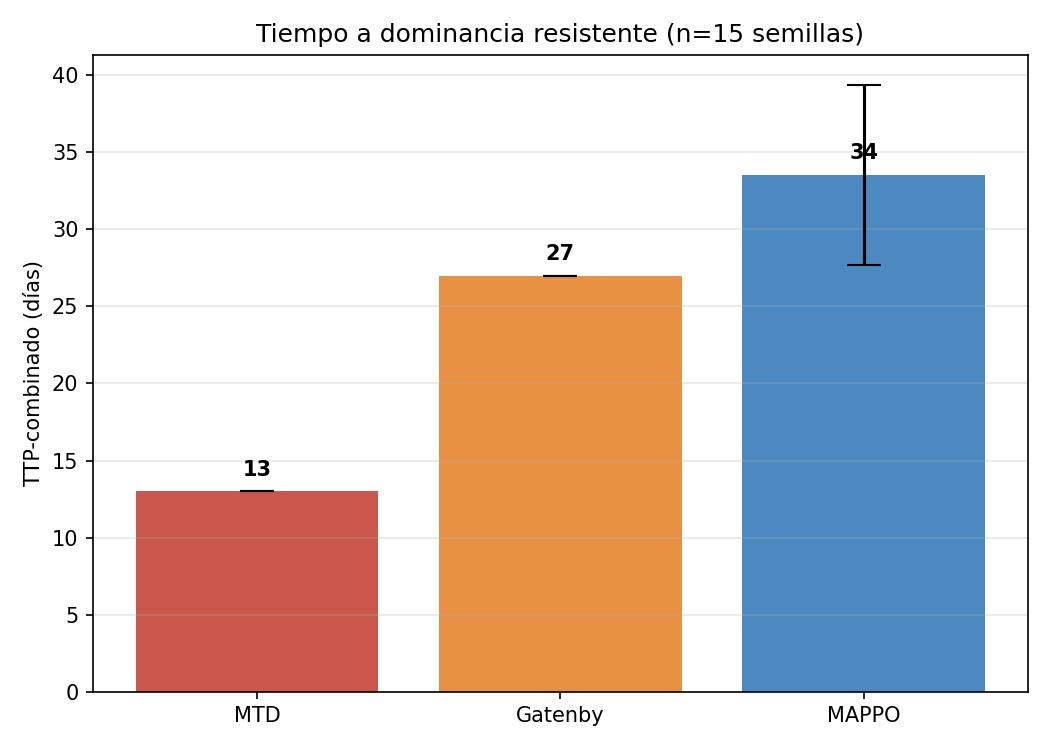
\includegraphics[width=0.6\textwidth]{images/validation_seeds.png}
\caption{Validación multi-semilla del TTP-combinado ($n=15$). La política aprendida supera a ambas líneas base deterministas; la barra de error refleja la dispersión bimodal del self-play.}
\label{fig:validation}
\end{figure}

\section{Mecanismo de la política aprendida}
\label{sec:res-mecanismo}

La inspección de las políticas de la cuenca superior revela el mecanismo descubierto por el agente. La Figura~\ref{fig:mecanismo} muestra que la política aplica una \textbf{dosificación pulsada e intermitente}: tras un periodo inicial, la dosis oscila entre valores bajos y nulos en lugar de mantenerse al máximo. Como consecuencia, la población sensible se mantiene en una densidad elevada que compite con la resistente y frena su expansión, mientras la fracción resistente crece lentamente hasta cruzar el umbral de mayoría. Este patrón corresponde al principio de la terapia adaptativa ---preservar una población sensible competidora--- redescubierto de forma autónoma por el agente, sin haber sido programado explícitamente.

\begin{figure}[H]
\centering
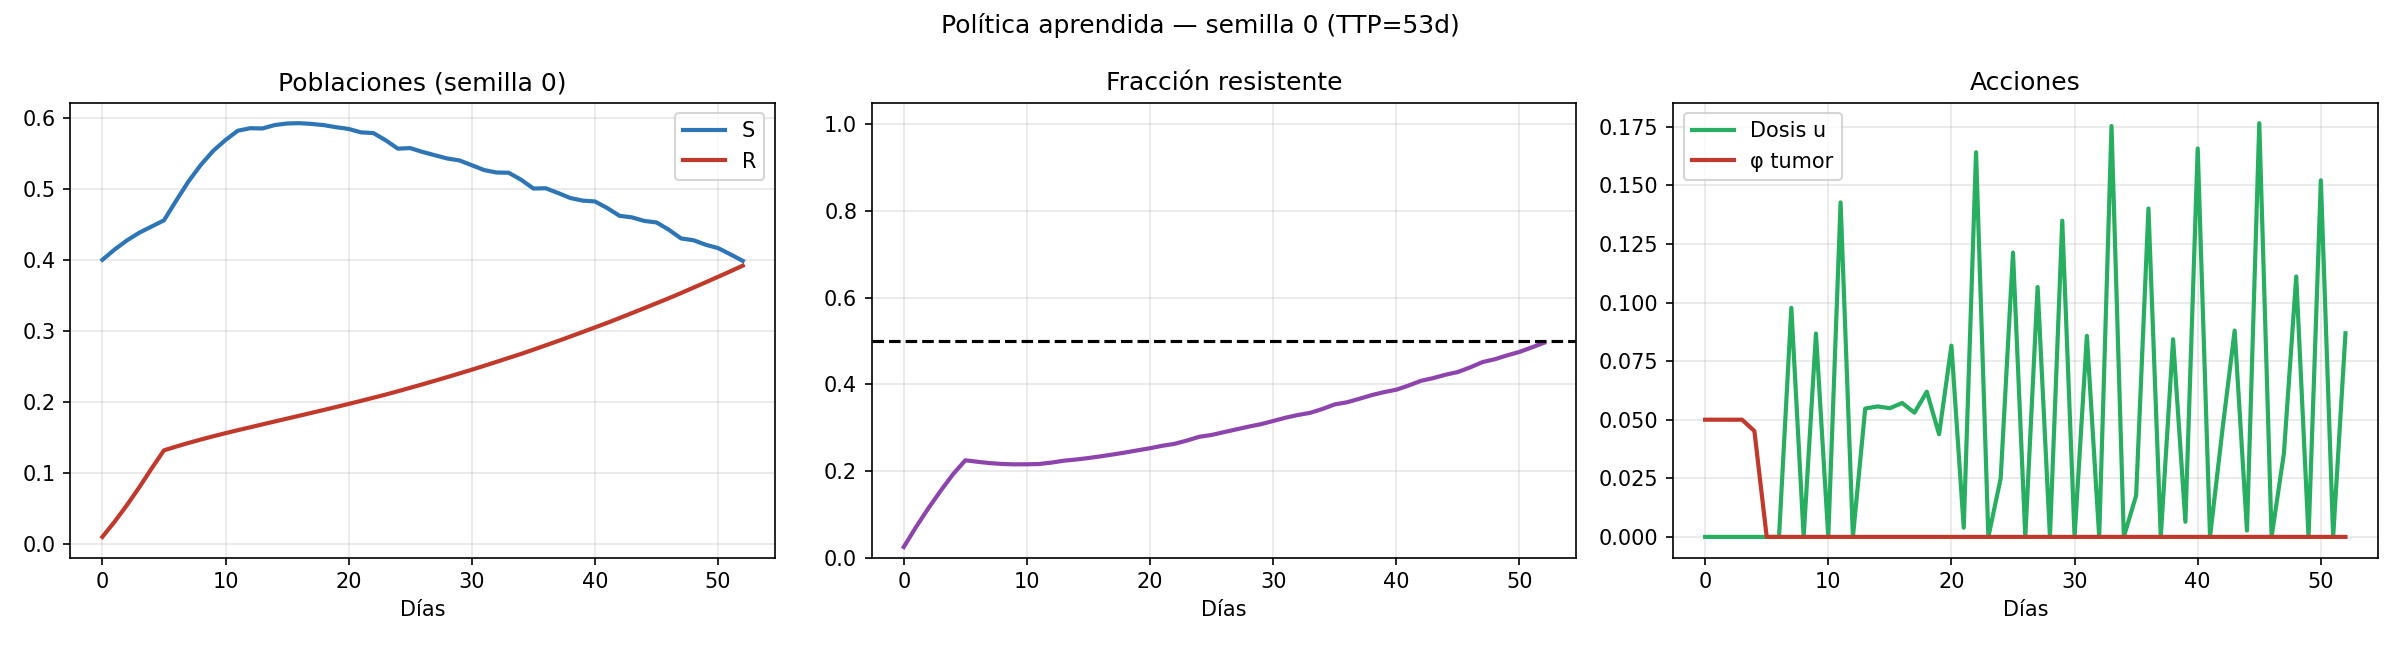
\includegraphics[width=0.95\textwidth]{images/policy_seed0.png}
\caption{Política aprendida de la cuenca superior: poblaciones (izquierda), fracción resistente (centro) y acciones de dosis y transición (derecha). La dosificación pulsada preserva la población sensible competidora.}
\label{fig:mecanismo}
\end{figure}

\section{Ablación del crítico centralizado (CTDE vs.\ IPPO)}
\label{sec:res-ablacion}

Para aislar la contribución del crítico centralizado, se comparó MAPPO (crítico condicionado al estado conjunto) con IPPO (crítico con observación local), manteniendo idénticos el actor, la observación de ejecución y todos los hiperparámetros. La verificación de la arquitectura confirmó que el cambio de variante modifica efectivamente la dimensión de entrada del crítico (3 para MAPPO, 2 para IPPO).

Bajo la métrica auditada y la calibración nueva, MAPPO alcanza una mediana de 34 días frente a 31 días de IPPO en quince pares de semillas (Tabla~\ref{tab:res-ablacion}). El contraste Wilcoxon pareado unilateral MAPPO$>$IPPO da $p=0{,}013759$; debe considerarse evidencia exploratoria condicionada al simulador. En esta corrida, las quince políticas IPPO fallaron por carga, mientras que MAPPO falló por resistencia en seis semillas y por carga en nueve.

\begin{table}[H]
\centering
\caption{Ablación calibrada del crítico centralizado ($n=15$). Ambas variantes comparten actor, observación de ejecución e hiperparámetros; solo difiere la entrada del crítico.}
\label{tab:res-ablacion}
\renewcommand{\arraystretch}{1.25}
\begin{tabular}{l|c|l}
\textbf{Variante} & \textbf{TTP (días)} & \textbf{Modo de falla} \\
\hline
MAPPO (crítico centralizado, CTDE) & $34$ [27,41] & 6 resistencia, 9 carga \\
IPPO (crítico local)               & $31$ [23,34] & 15 carga \\
\end{tabular}
\end{table}

\begin{figure}[H]
\centering
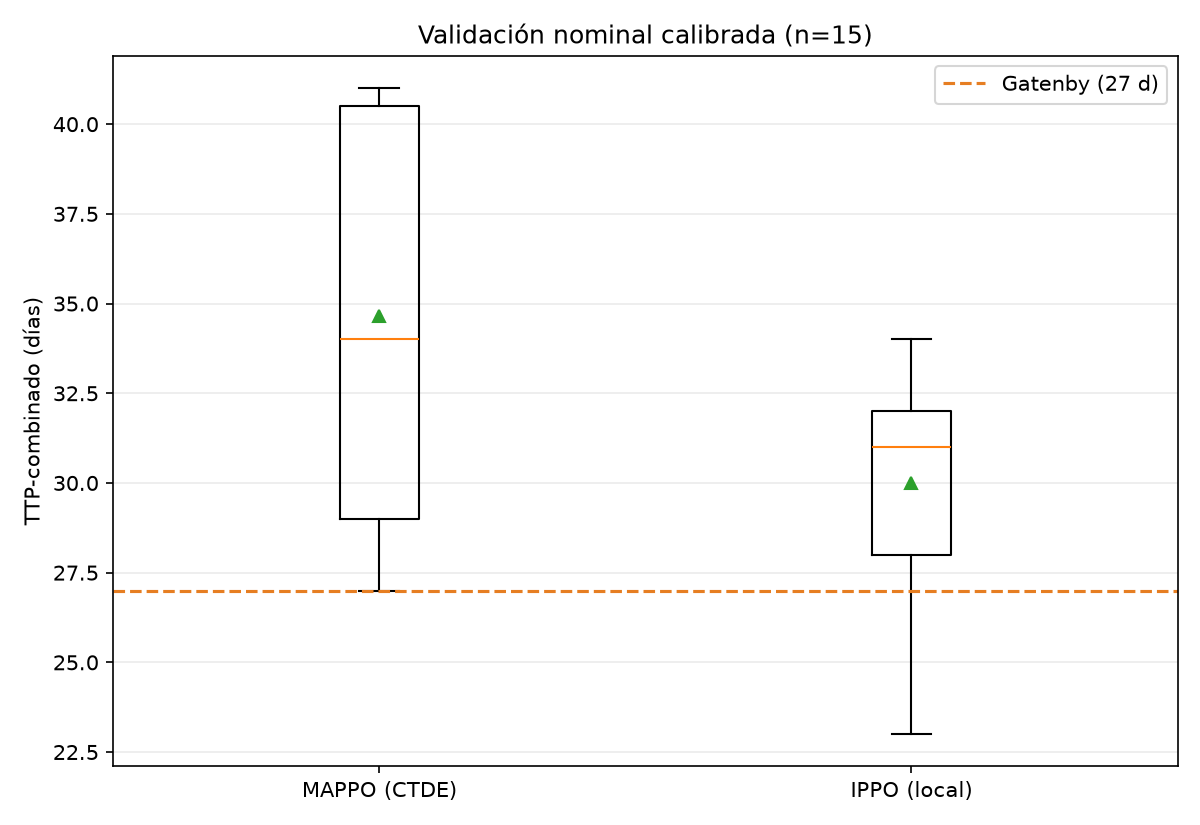
\includegraphics[width=0.6\textwidth]{images/ablation_ctde_15.png}
\caption{Ablación CTDE: MAPPO (crítico centralizado) frente a IPPO (crítico local) bajo el TTP-combinado.}
\label{fig:ablacion}
\end{figure}

\section{Análisis de sensibilidad}
\label{sec:res-sensibilidad}

En la auditoría calibrada se varió, una a la vez, cada una de las ocho constantes de dinámica y fármaco en factores de $0{,}8$ a $1{,}2$, manteniendo congeladas las políticas nominales. La Tabla~\ref{tab:res-sensibilidad} resume el rango del TTP-combinado de MAPPO sobre quince semillas. La política conserva una ventaja nominal en muchas perturbaciones, pero el ordenamiento $\text{MAPPO} > \text{Gatenby}$ no es universal: la reducción de $K$ y el aumento de $\mathrm{IC50}_S$ pueden eliminarla.

\begin{table}[H]
\centering
\caption{Análisis de sensibilidad calibrado. Rango del TTP-combinado de MAPPO sobre quince semillas al variar cada parámetro entre $0{,}8\times$ y $1{,}2\times$ su valor nominal.}
\label{tab:res-sensibilidad}
\renewcommand{\arraystretch}{1.25}
\begin{tabular}{l|c}
\textbf{Constante variada} & \textbf{MAPPO (rango, días)} \\
\hline
$\mathrm{IC50}_S$                  & 21--41 \\
$\mathrm{IC50}_R$                  & 27--41 \\
$\delta_S^{\max}$                 & 23--41 \\
$\delta_R^{\max}$                 & 26--41 \\
$\alpha_S$                         & 20--41 \\
$\alpha_R$                         & 26--45 \\
$\lambda_c$                        & 26--41 \\
$K$                                & 10--41 \\
\end{tabular}
\end{table}

El parámetro más sensible de esta corrida fue $K$: al reducirlo a $0{,}8K$, la mediana de MAPPO cayó a 25 días, frente a 34 días en el régimen nominal. También hubo degradación al aumentar $\mathrm{IC50}_S$ a $1{,}2\times$ (24 días) y $\alpha_S$ a $1{,}2\times$ (26 días). La Figura~\ref{fig:sensibilidad} muestra el barrido calibrado actualizado; los valores completos se conservan en el reporte de EXP-1.

\begin{figure}[H]
\centering
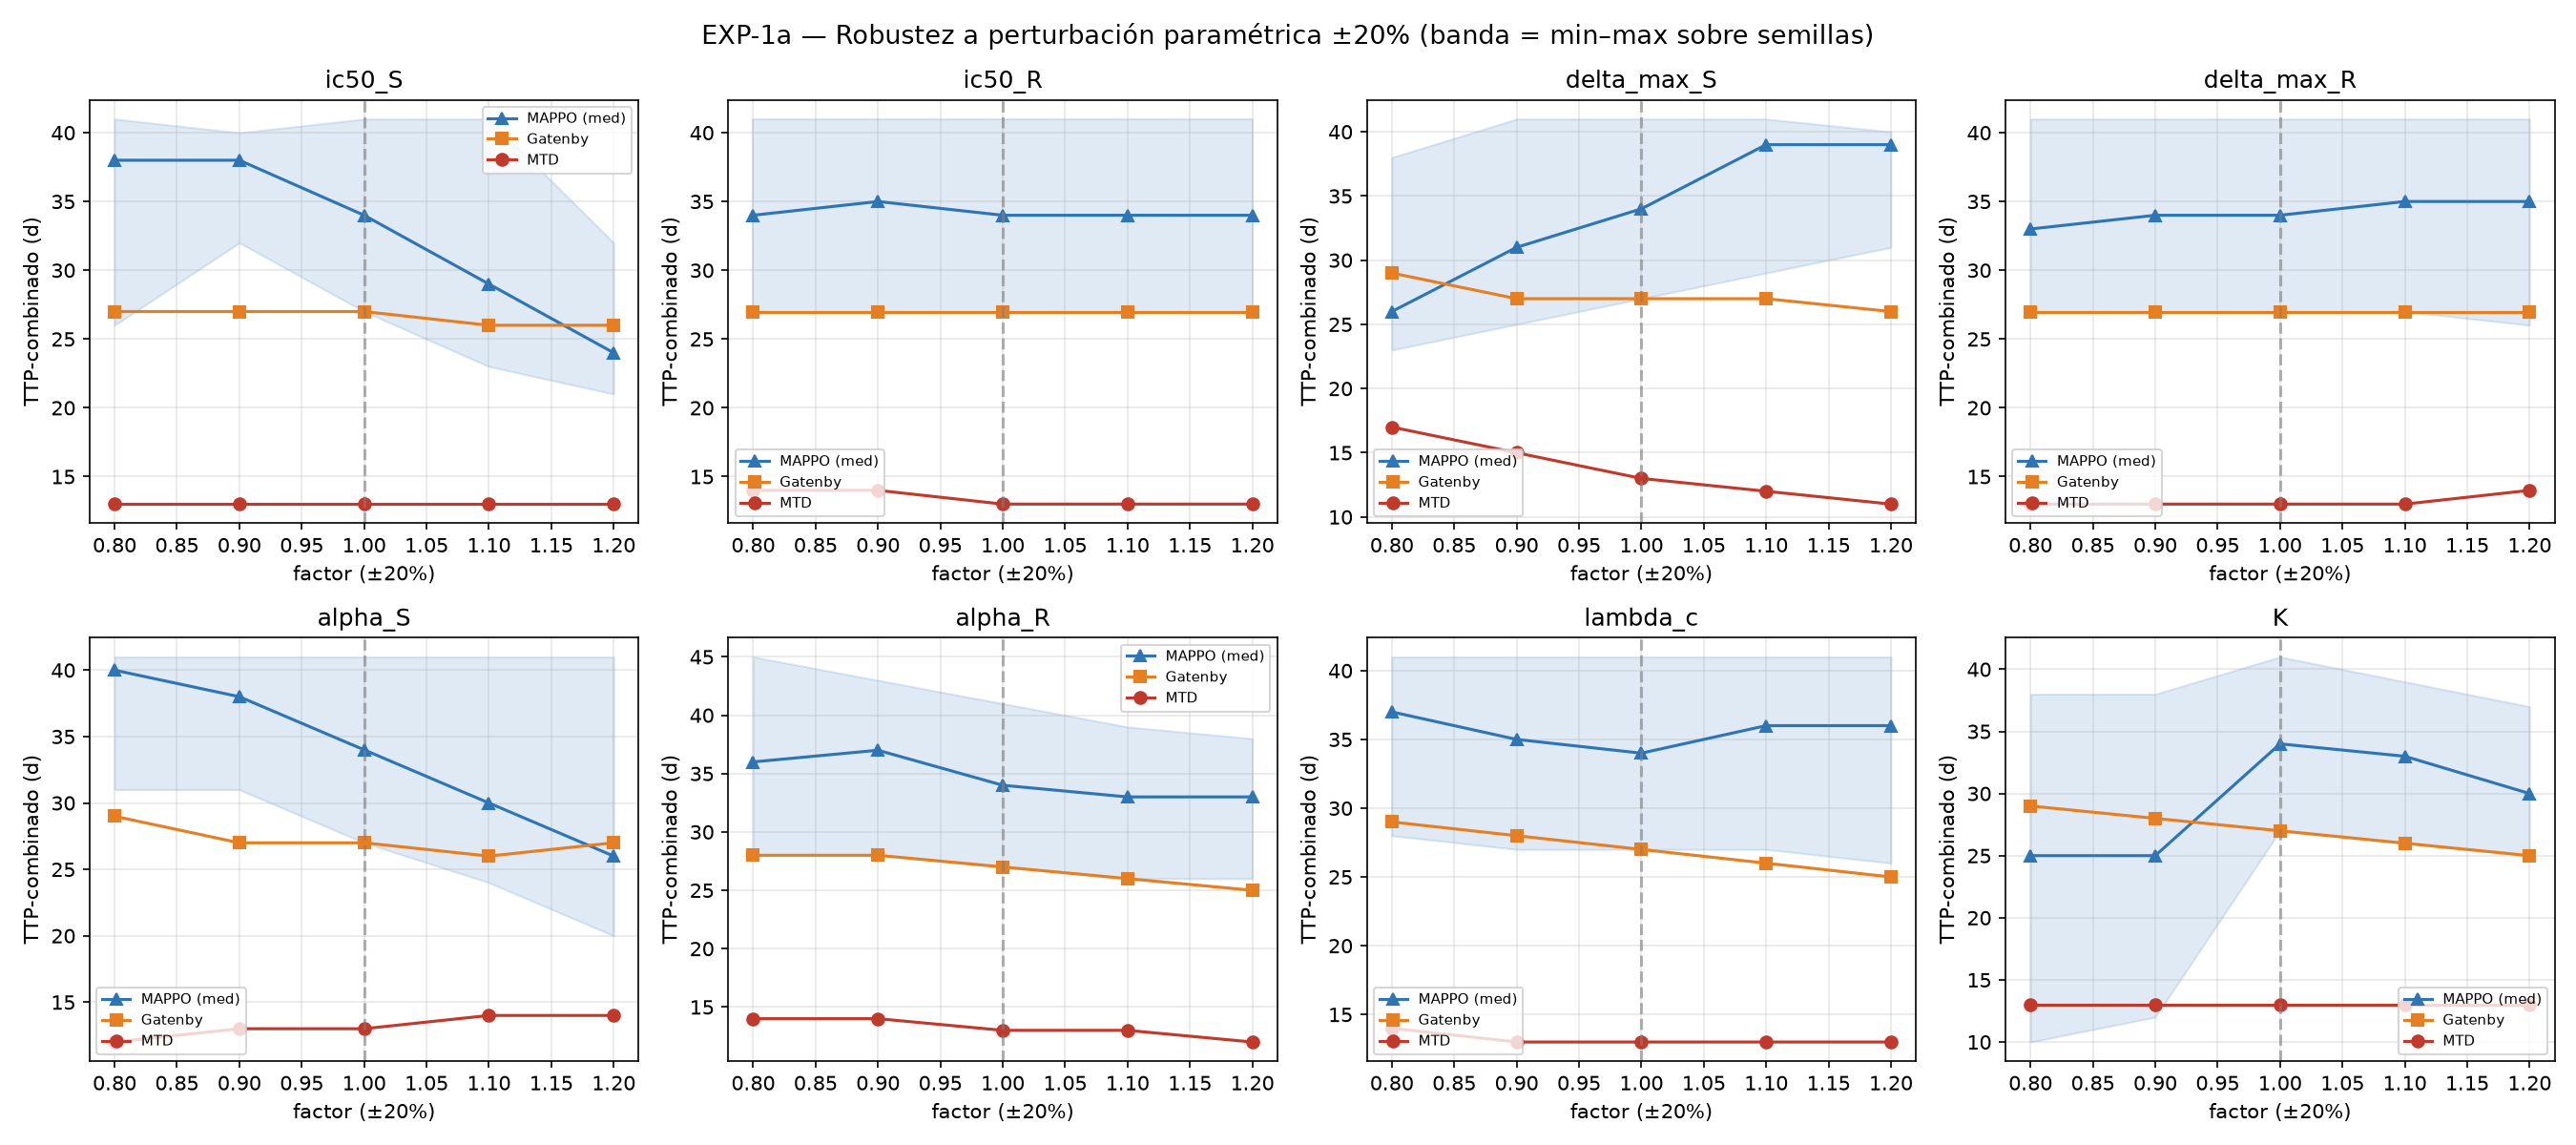
\includegraphics[width=0.95\textwidth]{images/exp1a_perturbacion_v2.png}
\caption{Análisis de sensibilidad calibrado de EXP-1. Cada panel muestra la mediana y la banda mínimo--máximo del TTP-combinado de MAPPO sobre quince semillas, junto con MTD y Gatenby, al variar una constante entre $0{,}8\times$ y $1{,}2\times$.}
\label{fig:sensibilidad}
\end{figure}

\section{Confirmación con la corrida completa reproducible}
\label{sec:res-confirmacion}

Para verificar que los hallazgos no dependen de la maquinaria de cómputo, se reejecutó la comparación nominal con el arnés reanudable y checkpointing intra-corrida descrito en la Sección~\ref{sec:checkpointing}. MAPPO e IPPO se entrenaron desde cero con el mismo presupuesto solicitado de \textbf{120\,000 pasos} (el último bloque produjo 120\,832 pasos), con \textbf{quince semillas independientes} por variante, usando la calibración real de DepMap/GDSC2. La evaluación se realizó con \texttt{TumorEnv} y $\phi=0{,}01$. Las líneas base, al ser deterministas, reprodujeron sus valores de forma exacta (sin tratamiento 12 días, MTD 13 días, Gatenby 27 días).

La Tabla~\ref{tab:res-confirmacion} reporta el resumen de las quince semillas; el detalle por semilla se conserva en el artefacto reproducible. La lectura principal es la \textbf{mediana}, el rango, los modos de falla y la tasa de éxito. MAPPO-CTDE alcanza 34 días [27--41] y supera a Gatenby en 13/15 semillas; IPPO alcanza 31 días [23--34] y lo hace en 12/15. El contraste Wilcoxon pareado unilateral MAPPO$>$IPPO da $p=0{,}013759$; se interpreta como evidencia exploratoria del simulador, no como eficacia clínica. El orden de medianas $\text{MAPPO} > \text{IPPO} > \text{Gatenby} > \text{MTD} > \text{Sin tratar}$ se observa en esta corrida.

\begin{table}[H]
\centering
\caption{Corrida calibrada reproducible (presupuesto solicitado de 120\,000 pasos; 120\,832 pasos efectivos; $n=15$ semillas por variante). TTP-combinado, modos de falla y tasa de éxito frente a Gatenby (27 días).}
\label{tab:res-confirmacion}
\renewcommand{\arraystretch}{1.25}
\resizebox{\textwidth}{!}{%
\begin{tabular}{l|c|l|c}
\textbf{Variante} & \textbf{TTP mediana [min,max]} & \textbf{Modo de falla} & \textbf{Éxito $>$Gatenby} \\
\hline
MAPPO (CTDE) & \textbf{34 [27,41]} & 6 resistencia, 9 carga & \textbf{13/15} \\
IPPO (local) & \textbf{31 [23,34]} & 15 carga & 12/15 \\
\end{tabular}
}
\end{table}

En la corrida actual, las dosis medias fueron aproximadamente 0.056 para MAPPO y 0.064 para IPPO. Este patrón es compatible con dosificación de baja intensidad, pero no basta por sí solo para afirmar un mecanismo clínico. El detalle por semilla y los checkpoints están en el reporte reproducible del repositorio; la figura calibrada se muestra a continuación.

\begin{figure}[H]
\centering
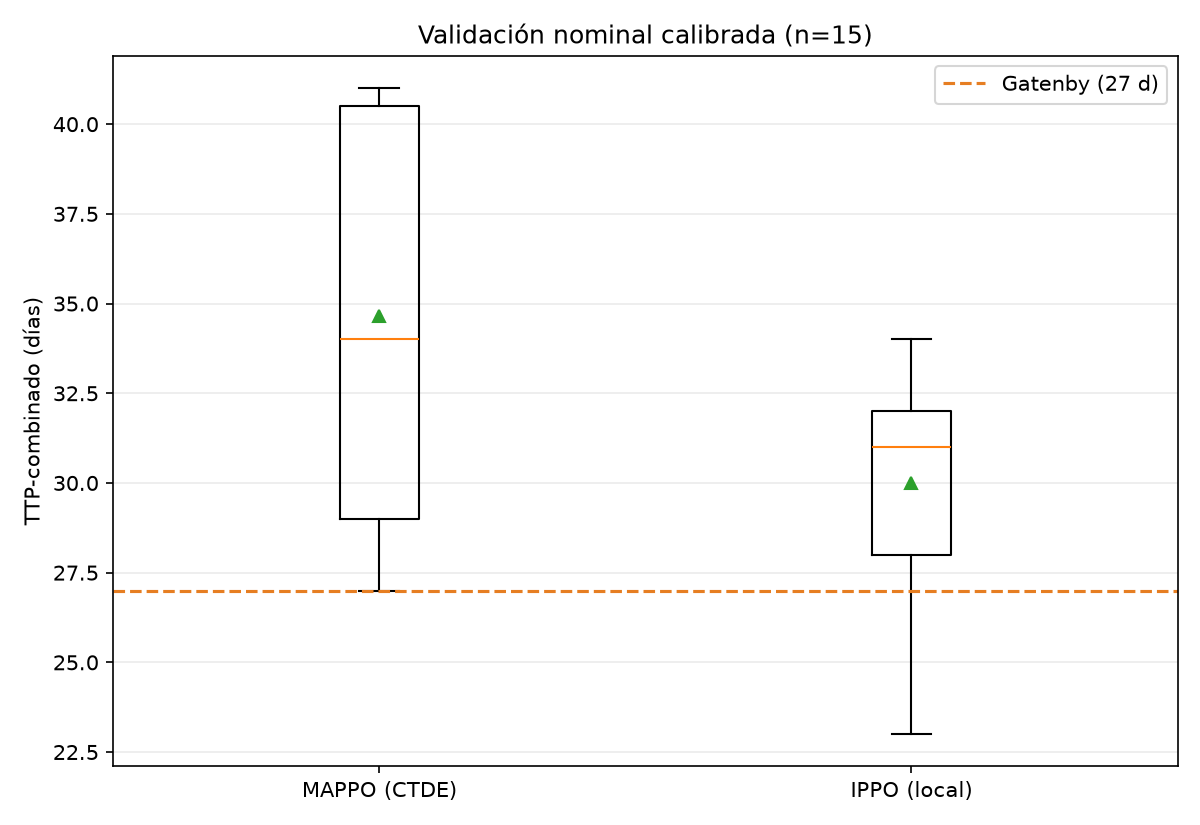
\includegraphics[width=0.72\textwidth]{images/validacion_calibrada_15semillas.png}
\caption{Validación nominal calibrada con quince semillas. La línea discontinua indica el TTP determinista de Gatenby (27 días); los puntos medios muestran la media de cada distribución.}
\label{fig:validation-calibrated}
\end{figure}

\subsection{Control de censura con horizonte extendido}

Para verificar que los tiempos reportados no fueran simplemente un tope impuesto por el
horizonte administrativo, se repitió la evaluación representativa con un horizonte de
360 días, conservando la calibración real, el adversario fijo y el TTP-combinado. Los
episodios sin tratamiento, MTD, Gatenby y MAPPO terminaron por carga o resistencia en
12, 13, 27 y 41 días, respectivamente. Ninguno alcanzó el día 360: los resultados son
fallos observados y no observaciones censuradas por el horizonte.

\subsection{EXP-2: adversario tumoral fortalecido}
\label{sec:res-exp2}

El segundo experimento examinó si la comparación MAPPO--IPPO se mantiene cuando el
agente tumoral dispone de un rango de acción mayor. Se evaluaron tres regímenes,
$\phi_{max}\in\{0{,}05,0{,}10,0{,}20\}$, con quince semillas por método y régimen
(90 celdas de 120\,000 pasos). Cada política se enfrentó al tumor adaptativo
co-entrenado de su propia celda; Gatenby se evaluó contra ese mismo tumor. Por tanto,
la prueba mide robustez frente a un adversario endógeno comparable, no una cota
matemática del peor caso.

La Tabla~\ref{tab:res-exp2} resume la corrida completa. MAPPO supera a IPPO con el
adversario nominal ($\phi_{max}=0{,}05$), pero la diferencia desaparece al ampliar el
rango de acción tumoral. La lectura es importante: la ventaja de CTDE es dependiente
del régimen y no debe presentarse como una propiedad universal del método.

\begin{table}[H]
\centering
\caption{EXP-2 calibrado: TTP-combinado frente al tumor adaptativo co-entrenado,
mediana [mín, máx], quince semillas por celda. Los valores $p$ son Wilcoxon pareado
unilateral MAPPO$>$IPPO, con corrección de Holm entre los tres regímenes.}
\label{tab:res-exp2}
\renewcommand{\arraystretch}{1.2}
\resizebox{\textwidth}{!}{%
\begin{tabular}{c|c|c|c|c|c|c}
\textbf{$\phi_{max}$} & \textbf{MAPPO} & \textbf{IPPO} & \textbf{$p$} & \textbf{Holm $p$} & \textbf{Éxito M} & \textbf{Éxito I} \\
\hline
0,05 & \textbf{44 [24,58]} & 29 [26,37] & 0,005 & 0,014 & 15/15 & 13/15 \\
0,10 & 28 [22,47] & 27 [23,35] & 0,648 & 0,648 & 15/15 & 14/15 \\
0,20 & 24 [21,50] & 26 [20,34] & 0,265 & 0,530 & 15/15 & 15/15 \\
\end{tabular}}
\end{table}

El modo de falla de MAPPO fue carga en 11/15, 15/15 y 13/15 semillas para los tres
regímenes, respectivamente, y resistencia en las restantes. IPPO terminó por carga
en las 45 semillas. Esto muestra además que fortalecer al adversario cambia no solo
el TTP, sino también qué límite del sistema se alcanza primero. Los resultados son
evidencia in silico de sensibilidad al régimen adversarial; no implican eficacia
clínica ni permiten afirmar que un adversario aprendido sea óptimo.

\begin{figure}[H]
\centering
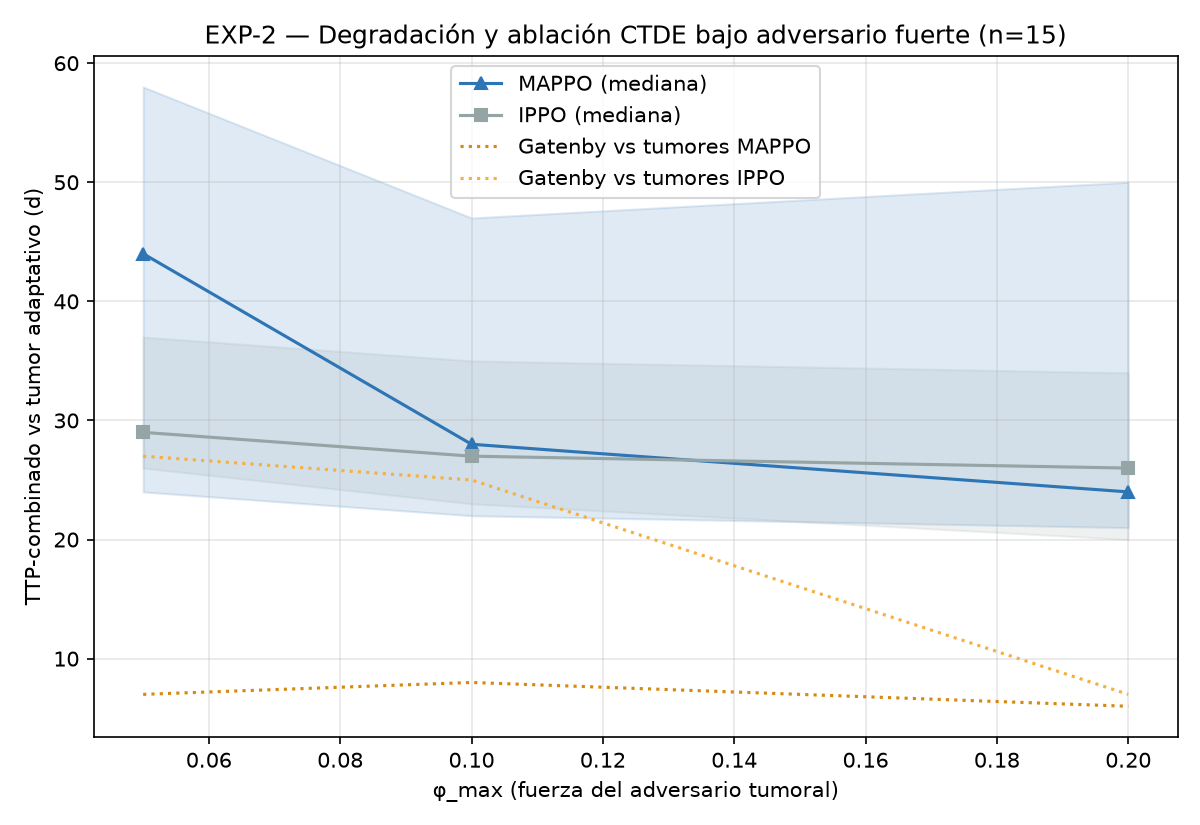
\includegraphics[width=0.78\textwidth]{images/exp2_adversario_v2.png}
\caption{EXP-2 calibrado. La mediana y el rango del TTP-combinado de MAPPO e IPPO
se muestran al aumentar el límite de transición tumoral $\phi_{max}$.}
\label{fig:exp2-adversario}
\end{figure}

\section{Robustez adversarial mediante explotabilidad}
\label{sec:res-explotabilidad}

Un juego resuelto por \textit{self-play} puede sobreajustarse al adversario con el que
co-evolucionó. Para examinar esta posibilidad se evaluó la \textbf{explotabilidad} de
cada política, siguiendo el estándar de la teoría de juegos computacional~\cite{deWitt2020}.
Se congeló cada terapia, se entrenaron cinco adversarios tumorales dedicados desde
reinicios independientes y se conservó el más dañino. La corrida titular usó quince
semillas, $\phi_{max}=0{,}05$ y 120\,000 pasos. La explotabilidad se define como
$\text{TTP}_{self-play}-\text{TTP}_{best-response}$; una brecha menor indica menor
degradación ante el atacante dedicado. PPO no garantiza el óptimo global, por lo que
estos resultados son una estimación empírica y no una cota matemática del peor caso.

\begin{table}[H]
\centering
\caption{Benchmark V2 calibrado ($n=15$ semillas, cinco reinicios de \textit{best-response}). Se reporta la mediana [mín, máx] del TTP-combinado frente al tumor de \textit{self-play}, frente al mejor atacante dedicado y la brecha de explotabilidad. Gatenby, sometido a cinco reinicios análogos, obtuvo 7 días.}
\label{tab:res-explotabilidad}
\renewcommand{\arraystretch}{1.25}
\resizebox{\textwidth}{!}{%
\begin{tabular}{l|c|c|c|c}
\textbf{Variante} & \textbf{TTP self-play} & \textbf{TTP best-response} & \textbf{Explotabilidad} & \textbf{TTP $>$ 7 d} \\
\hline
MAPPO (CTDE) & $44\ [24,58]$ & $\mathbf{14\ [11,14]}$ & $30\ [11,44]$ & 15/15 \\
IPPO (local) & $29\ [26,37]$ & $11\ [10,12]$          & $18\ [14,27]$ & 15/15 \\
\end{tabular}
}%
\end{table}

La terapia MAPPO conserva un TTP absoluto mayor frente al mejor atacante encontrado
(14 frente a 11 días), pero también presenta una brecha puntual mayor (30 frente a
18 días). El contraste unilateral preespecificado para la hipótesis
$\text{explotabilidad}_{MAPPO}<\text{explotabilidad}_{IPPO}$ no respalda esa dirección
($p=0{,}993$); por tanto, no se afirma que MAPPO sea menos explotable. El resultado sí
obliga a separar dos ideas: un TTP absoluto más alto no equivale automáticamente a una
menor sensibilidad a un atacante dedicado.

El cross-play aporta una prueba fuera del compañero de entrenamiento: MAPPO frente a
la población de tumores IPPO obtuvo 35 días [24,41], mientras IPPO frente a tumores
MAPPO obtuvo 27 días [12,29]. La asimetría sugiere mejor transferencia de MAPPO en
este escenario, aunque no constituye por sí sola una prueba de significancia ni de
robustez universal.

\begin{figure}[H]
\centering
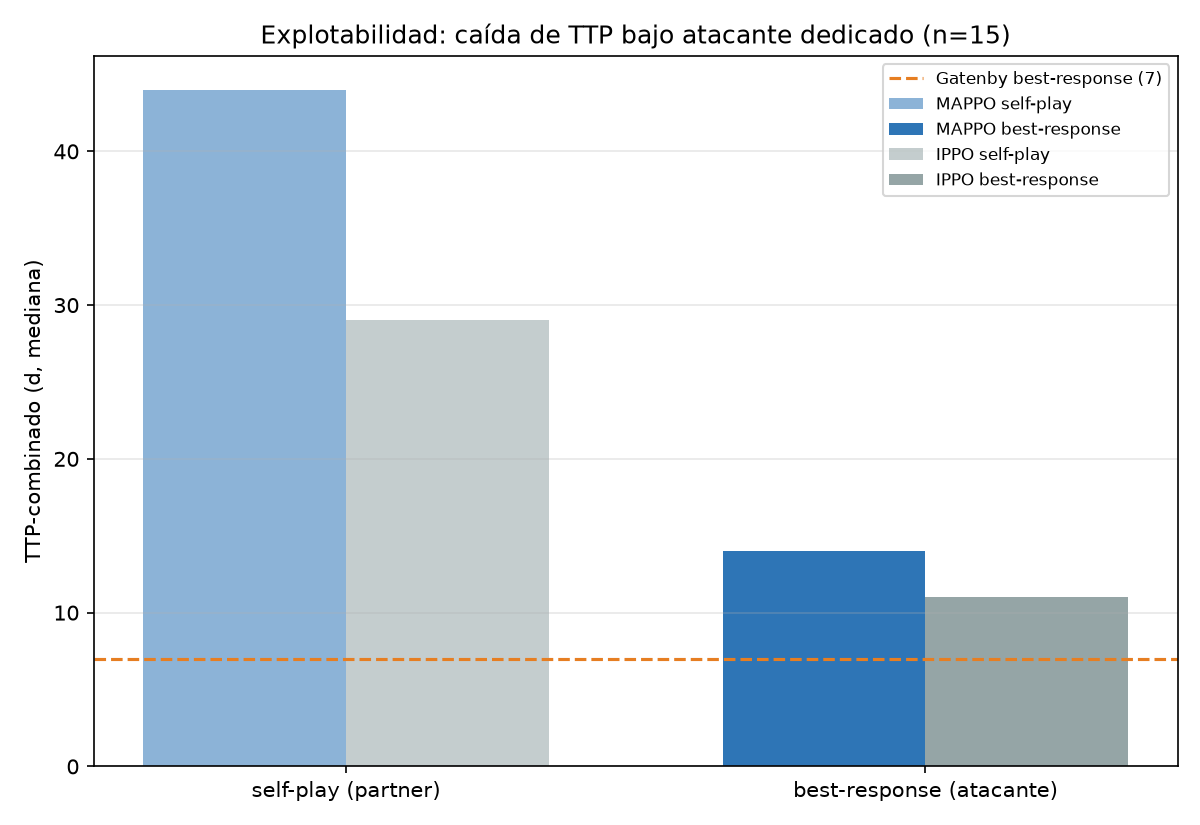
\includegraphics[width=0.7\textwidth]{images/benchmark_exploit_v2.png}
\caption{Benchmark V2: TTP-combinado de self-play y frente al mejor atacante dedicado
para MAPPO e IPPO. La línea de Gatenby corresponde a su propia best-response aproximada.}
\label{fig:explotabilidad}
\end{figure}

En conjunto, la auditoría calibrada muestra que la política aprendida extiende el tiempo
de manejo simulado frente a MTD y Gatenby en el escenario nominal, con una ventaja de
MAPPO sobre IPPO en la comparación nominal y en cross-play. EXP-2 muestra, sin embargo,
que esa ventaja desaparece al fortalecer el adversario; el benchmark V2 muestra además
que el TTP absoluto y la explotabilidad son propiedades distintas. Por tanto, el
resultado debe interpretarse como evidencia \textit{in silico} de comportamiento
adaptativo bajo el modelo especificado, no como eficacia clínica ni como robustez
universal.

\customchapter{CONCLUSIONES}
\label{cap:conclusiones}

Esta tesis diseñó y evaluó GBMARL, un marco de aprendizaje por refuerzo multiagente adversarial para estudiar la dosificación adaptativa de temozolomida frente a la resistencia evolutiva del glioblastoma. La conclusión principal es que el marco puede descubrir políticas que retrasan el tiempo a falla en el escenario nominal del simulador, pero la magnitud de esa ventaja depende de los supuestos biológicos, del endpoint y de la semilla de entrenamiento.

\section*{Conclusiones principales}
\phantomsection
\addcontentsline{toc}{subsection}{Conclusiones principales}

\begin{enumerate}
  \item \textbf{La calibración quedó trazable, pero no es una calibración clínica completa.} La integración de DepMap Public 26Q1 con GDSC2 release 8.5 recuperó 34 líneas GBM con ensayos de sensibilidad y 24 con expresión completa. La brecha estimada de sensibilidad a TMZ fue de aproximadamente 9,1 veces entre las poblaciones sensible y resistente. Esta evidencia informa la potencia relativa del fármaco; las tasas de crecimiento, la capacidad de carga y otros parámetros continúan siendo supuestos de literatura o de normalización y están identificados como tales.

  \item \textbf{El TTP-combinado distingue dos mecanismos de fracaso que antes podían confundirse.} La ausencia de tratamiento falló por carga en el día 12, mientras que MTD y Gatenby fallaron por mayoría resistente en los días 13 y 27. La política MAPPO de la evaluación representativa llegó al día 41 y falló por resistencia. Así, una carga final baja no se interpreta automáticamente como éxito: también se verifica si el tumor ya es predominantemente resistente.

  \item \textbf{MAPPO mostró una ventaja nominal sobre las líneas base en la corrida calibrada.} En quince semillas, MAPPO obtuvo mediana 34 [27, 41] días y superó a Gatenby en 13/15 semillas. IPPO obtuvo mediana 31 [23, 34] días y superó a Gatenby en 12/15. La diferencia MAPPO--IPPO fue compatible con una ventaja del crítico centralizado en esta muestra ($p=0{,}013759$), pero sigue siendo evidencia \emph{in silico} condicionada al simulador y no eficacia clínica.

  \item \textbf{La sensibilidad delimita la afirmación.} El análisis OAT de ocho parámetros mostró que la ventaja no es universal. La reducción de la capacidad de carga fue especialmente crítica: con $K=0{,}8K_0$, la mediana de MAPPO cayó a 25 días frente a 34 días nominales. En una perturbación conjunta de factores entre 0,8 y 1,2, la mediana de las medianas fue 30 días, pero existieron entornos donde la tasa de éxito frente a Gatenby fue 0\,\%. El hallazgo es, por tanto, una propiedad del régimen modelado y no una garantía ante cualquier paciente o tumor.

  \item \textbf{El pipeline es reproducible y auditable.} Se corrigió el filtrado de perfiles de expresión de DepMap, se documentaron hashes y procedencia, se verificó la equivalencia numérica entre el entorno rápido y el de referencia, y la suite de regresión terminó con 26 pruebas aprobadas. El entrenamiento se ejecutó con quince semillas por variante y 120\,832 pasos efectivos, conservando checkpoints reanudables.
\end{enumerate}

\section*{Respuesta a la pregunta de investigación}
\phantomsection
\addcontentsline{toc}{subsection}{Respuesta a la pregunta de investigación}

Bajo la calibración, el endpoint y el adversario fijo especificados, GBMARL sí permitió descubrir una política MAPPO con mayor TTP nominal que MTD y Gatenby, y la comparación MAPPO--IPPO sugiere que el crítico centralizado puede mejorar el resultado en este entorno. Sin embargo, la evidencia disponible no autoriza afirmar superioridad universal, robustez frente a un adversario óptimo ni eficacia clínica. La respuesta correcta es condicional: el método es prometedor como marco computacional y su valor depende de que los parámetros, la fuerza adversarial y los criterios de progresión estén bien justificados.

\section*{Limitaciones finales}
\phantomsection
\addcontentsline{toc}{subsection}{Limitaciones finales}

El modelo no incluye espacio, heterogeneidad clonal detallada, farmacocinética clínica, radioterapia, combinaciones terapéuticas ni una cohorte de pacientes. La variable de salud del paciente tampoco debe interpretarse todavía como resultado clínico: sin datos de toxicidad longitudinal y una función de utilidad validada, solo puede permanecer como extensión experimental parametrizada. Además, EXP-2 permanece parcial: se han auditado 4 de 90 celdas, todas MAPPO con $\phi_{\max}=0{,}05$; los niveles $0{,}10$ y $0{,}20$ y las celdas IPPO no deben presentarse como resultados actuales.

En conjunto, la tesis entrega un marco ejecutable, una métrica que separa carga y resistencia, una calibración farmacológica trazable y evidencia experimental reproducible con límites explícitos. Su contribución central no es afirmar que una política computacional ya sea un tratamiento, sino mostrar cómo evaluar de manera más honesta políticas adaptativas en presencia de resistencia evolutiva.

\chapter*{\center \Large RECOMENDACIONES}
\addcontentsline{toc}{section}{\bfseries RECOMENDACIONES}
\markboth{RECOMENDACIONES}{RECOMENDACIONES}

\begin{enumerate}
  \item \textbf{Conservar la validación multi-semilla como resultado principal.} La corrida nominal vigente usa 15 semillas por variante con huella de calibración fija, horizonte y endpoint explícitos. Para una conclusión más estrecha, añadir intervalos de confianza y más semillas sin reemplazar la mediana, el rango y los modos de falla.

  \item \textbf{Evaluar frente a una población común de adversarios.} EXP-2 ya completó las 90 celdas previstas. La siguiente ampliación debe comparar MAPPO, IPPO y las líneas base frente a los mismos adversarios reservados para evaluación, además de los compañeros de self-play, para reducir la confusión entre la calidad de la terapia y la dificultad del tumor co-entrenado.

  \item \textbf{Ampliar la verificación del atacante.} El benchmark V2 ya incluye cinco reinicios por terapia, el compañero de self-play y cross-play. Una ampliación útil es medir la estabilidad del peor TTP encontrado al variar el presupuesto de entrenamiento y los reinicios; la mejor respuesta aproximada obtenida no garantiza un óptimo global.

  \item \textbf{Mejorar la calibración biológica.} Separar en el reporte qué parámetros provienen de datos, cuáles de literatura y cuáles de normalización. Cuando sea posible, incorporar curvas dosis--respuesta por línea, incertidumbre bootstrap, datos temporales de crecimiento y mediciones de eliminación del fármaco, en lugar de tratar la brecha de IC50 como identificación completa de la dinámica.

  \item \textbf{Implementar la salud del paciente como un módulo validado, no como una penalización arbitraria.} La salud debe representar variables observables y clínicamente interpretables, por ejemplo toxicidad hematológica acumulada, función orgánica y calidad de vida. Cada componente necesita escala, horizonte temporal, umbral y fuente de calibración; la recompensa debe incluir una restricción o presupuesto de toxicidad separado del TTP. Hasta contar con esos datos, la salud debe permanecer como análisis de sensibilidad y no como conclusión clínica.

  \item \textbf{Ampliar la evaluación externa.} Comparar las políticas con control óptimo, búsqueda evolutiva y otros algoritmos de RL; realizar validación fuera de muestra por línea celular; y probar escenarios con variabilidad de parámetros, observación parcial, retrasos de medición y errores de adherencia. Estas pruebas ayudarán a distinguir una política que aprendió una estrategia general de una que explotó una regularidad particular del simulador.

  \item \textbf{Mantener la trazabilidad de resultados.} Cada tabla o figura debe indicar la fecha, la huella de calibración, el número de semillas, el adversario, el horizonte y si el resultado es histórico, parcial o vigente. Los artefactos históricos no deben mezclarse con la corrida calibrada actual.
\end{enumerate}
 % sección opcional

%% ============================================================================
\renewcommand{\bibname}{\hfill\Large\bf{REFERENCIAS BIBLIOGRÁFICAS}\hfill}

\bibliographystyle{IEEEtran} % Estableciendo el estilo de citas IEEEtram.

\bibliography{referencias} % Recibe las referencias de IEEE

\input{secciones/anexos}

\end{document}
